\section{Methodology}
\label{cha:methodology}

\subsection{Twitter Covert Channel}
\label{sec:methodology:twittercc}

\subsubsection{The Stego System}
\label{subsec:methodology:twittercc:stego}

To perform the botnet command and control communication, a covert channel
(stego system) that communicates using the Twitter social network has been
developed.  This covert channel is similar to Desoky's \cite{nostega} noiseless
steganography and utilizes the cover generation paradigm, however there are some differences.
Even in the noiseless steganography systems, the secret messages are
usually embedded in to the actual data of the cover objects.  For example, in
graph steganography, the plotted data contains the secret message.  In this
system, where the cover objects are tweets, the secret message is not contained
in the data of the tweet (the text), instead it is contained in the
\emph{metadata} of the tweet (the length).  Metadata refers to ``data about
data.''  All data has some metadata associated with it, but this metadata is not
explitictly stored.  It is inferred from the existing data.  The tweet's data is
the text.  The tweet also has metadata such as the time it was posted, the user
account, and the length of the text posted.  Additional metadata could include
the letter frequencies of the posted text or the number of spaces in the text.

Because this system differs from existing steganographic systems, we will
define the parts of this system as follows:

\begin{enumerate}
  \item The set of possible cover messages, $\mathcal{X}^*$, is the set of
  possible tweets, which is the set of messages of up to 140
  UTF-8\footnote{\url{https://dev.twitter.com/docs/counting-characters}}
  characters.
  \item The set of possible secret messages, $\mathcal{M}$, can be defined as
  $\Sigma^*$, where the $\Sigma$ notation is taken from the formal languages
  domain, and refers to an alphabet of symbols, where the symbols can be
  arbitrarily defined.  For example, one implementation may use $\Sigma = \{a,
  b, c, \ldots, z\}$ (the English alphabet).
  \item The set of possible keys, $\mathcal{K}$, is the set of numbers that can
  be valid pseudo-random keys for the implementation.  In our case,
  the implementation uses the Java programming language's
  \ttf{java.util.Random}\footnote{\url{http://docs.oracle.com/javase/8/docs/api/java/util/Random.html}}
  class, which uses 48 bit keys.
  \item The \ttf{Embed} and \ttf{Generate} functions are combined.
  In our implementation we generate reasonable cover messages to have appropriate
  metadata that contains the secret message.
  \item The \ttf{Extract} function will also require a \ttf{Decode} step,
  described below.
  \item For convenience, we will also use the following notation for the set of
  natural numbers up to 140: $\tl = \{1, 2, \ldots, 140\}$.  Similarly, if
  we use $\mathbb{N}_n$, it means the natural numbers from 1 to $n$.  Unless
  otherwise stated, we assume $0 \not\in \mathbb{N}$.
\end{enumerate}

The overall system is shown in figure \ref{fig:twittercc}, where the numbered
components were implemented for the channel.

\begin{figure}
\centering
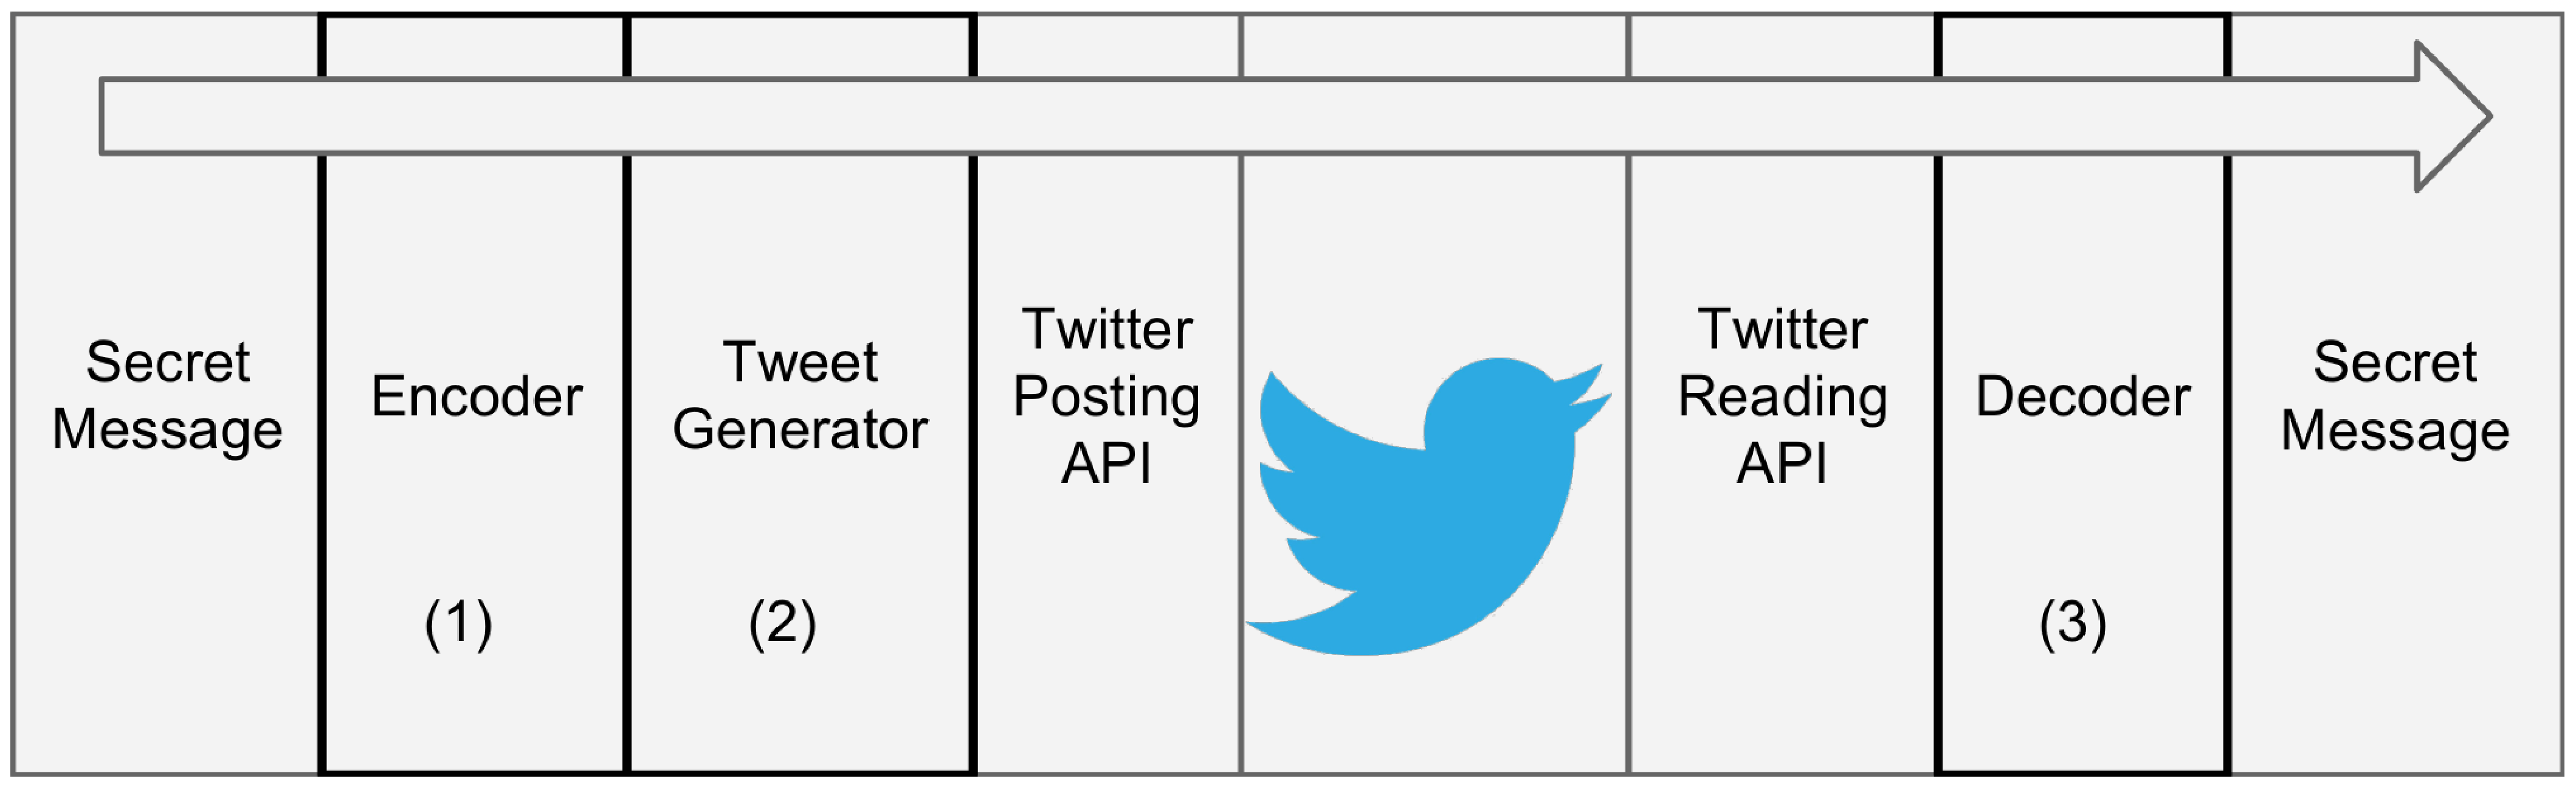
\includegraphics[width=\columnwidth]{twittercc.eps}
\caption{Overview of Twitter covert channel, where the numbered
components were implemented for the channel.}
\label{fig:twittercc}
\end{figure}

The secret message is embedded by utilizing the \emph{length} of the posted
tweets, by character count.  Because a tweet can have a length of up to 140
characters, the length value can store just over 7 bits of information per
tweet.  However, embedding 7 bits of information per tweet is not reasonable in
practice.  Certain length tweets rarely appear on Twitter so seeing, for
example, many tweets of length one or two on a single account would be
suspicious.  To solve these problems, we can use a one-to-many encoding
technique to hide information in the tweet lengths.  We will modify
the normal stego system definition to include the following functions:
\ttf{Encode}: $\mathcal{M} \times \mathcal{K} \rightarrow \tl$ and \ttf{Decode}:
$\tl \times \mathcal{K} \rightarrow \mathcal{M}$.  

\begin{figure}
\centering
\resizebox {\columnwidth} {!} {
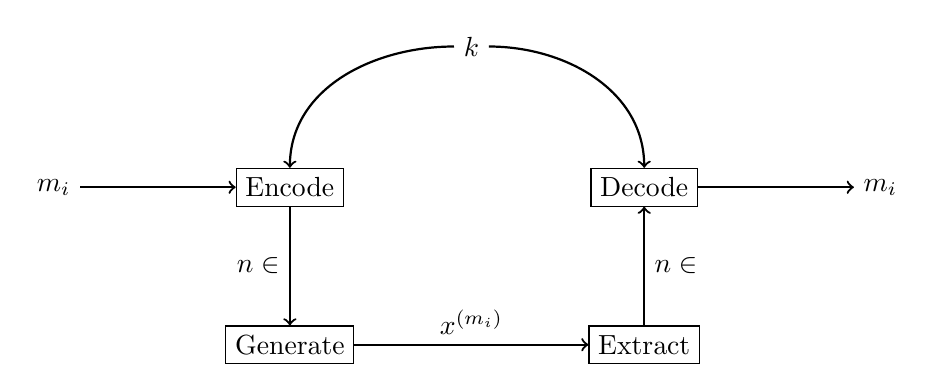
\begin{tikzpicture}
\node (m0) {$m_i$};
\node[draw] (encode) [right of=m0,node distance=3cm] {\ttf{Encode}};
\node[draw] (generate) [below of=encode,node distance=2cm] {\ttf{Generate}};
\node[draw] (extract) [right of=generate,node distance=4.5cm] {\ttf{Extract}};
\node[draw] (decode) [above of=extract,node distance=2cm] {\ttf{Decode}};
\draw[->,thick] (generate) -- (extract) node[pos=.5,above] (xm) {$x^{(m_i)}$};
\draw[->,thick] (encode) -- (generate) node[pos=.5,left] {$n \in \tl$};
\node (k) [above of=xm,node distance=3.5cm] {$k$};
\node (m1) [right of=decode,node distance=3cm] {$m_i$};
\draw[->,thick] (m0) -- (encode);
\draw[->,thick] (extract) -- (decode) node[pos=.5,right] {$n \in \tl$};
\path[->,thick] (k.west) edge [out=180,in=90] (encode.north);
\path[->,thick] (k.east) edge [out=0,in=90] (decode.north);
\draw[->,thick] (decode) -- (m1);
\end{tikzpicture}
}
\caption{Modified stego system diagram for Twitter covert channel.}
\label{fig:stego-twittercc}
\end{figure}

The modified stego system definition is shown in figure
\ref{fig:stego-twittercc}.  A message $m \in \mathcal{M}$ is broken up in to
symbols of $\Sigma$: $m_1m_2\ldots m_a$.  Each symbol $m_i$ is mapped to one of
several possible values using \ttf{Encode} along with the appropriate key $k$ to generate $n
\in \tl$, the appropriate tweet length value to use for this piece of the
message.  This value is passed to \ttf{Generate}, which generates a plausible
cover message $x^{(m_i)} \in \mathcal{X^*}$ to be posted to Twitter.  The
\ttf{Extract} function reads the posted tweets and calculates the length $n$ of
each tweet.  This value is passed to \ttf{Decode} along with the original key
$k$ to reconstruct the original message $m$ piece by piece.  This design assumes
that $\lvert\Sigma\rvert \leq 140$, and in fact, smaller alphabets should
improve the security of the channel.  A smaller alphabet allows mapping each symbol to more
possible length values, so repetitions of each length value are less likely.  We
will now present a simplified example to show the process of the stego
system.

\begin{example}[Encoding Table Generation]
\label{ex:methodology:twittercc:stego:encoding}
In this \\example, we will show the process for generating the encoding table.
Instead of using $\tl$ (all possible length values), we will use a reduced output
alphabet of $\mathbb{N}_{10}$ (1, 2, \ldots, 10) with an equal distribution.
For the input alphabet, we will use $\Sigma = \left\{a, b\right\}$ with an equal
distribution.

\begin{center}
\resizebox {\columnwidth} {!} {
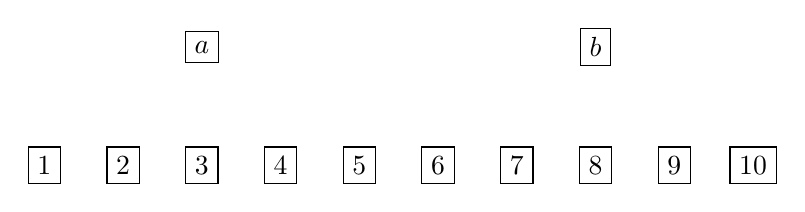
\begin{tikzpicture}
\node[draw] (a) {$a$};
\node[draw] (b) [right of=a,node distance=5cm] {$b$};

\node[draw] (3) [below of=a,node distance=1.5cm] {3};
\node[draw] (4) [right of=3,node distance=1cm] {4};
\node[draw] (5) [right of=4,node distance=1cm] {5};
\node[draw] (6) [right of=5,node distance=1cm] {6};
\node[draw] (7) [right of=6,node distance=1cm] {7};
\node[draw] (8) [right of=7,node distance=1cm] {8};
\node[draw] (9) [right of=8,node distance=1cm] {9};
\node[draw] (10) [right of=9,node distance=1cm] {10};
\node[draw] (2) [left of=3,node distance=1cm] {2};
\node[draw] (1) [left of=2,node distance=1cm] {1};
\end{tikzpicture}
}
\end{center}

First, choose one element of the output alphabet for each element
of $\Sigma$.  This guarantees that at least one output symbol will be mapped to
each input symbol.  Remove the chosen values of the output alphabet as options for
future choices.


\begin{center}
\resizebox {\columnwidth} {!} {
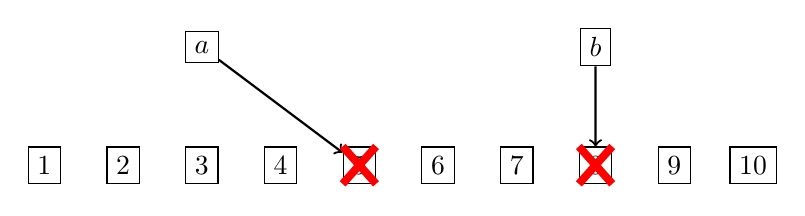
\begin{tikzpicture}
\node[draw] (a) {$a$};
\node[draw] (b) [right of=a,node distance=5cm] {$b$};

\node[draw] (3) [below of=a,node distance=1.5cm] {3};
\node[draw] (4) [right of=3,node distance=1cm] {4};
\node[draw] (5) [right of=4,node distance=1cm] {5};
\node[draw] (6) [right of=5,node distance=1cm] {6};
\node[draw] (7) [right of=6,node distance=1cm] {7};
\node[draw] (8) [right of=7,node distance=1cm] {8};
\node[draw] (9) [right of=8,node distance=1cm] {9};
\node[draw] (10) [right of=9,node distance=1cm] {10};
\node[draw] (2) [left of=3,node distance=1cm] {2};
\node[draw] (1) [left of=2,node distance=1cm] {1};

\draw[->,thick] (a) -- (5);
\draw[->,thick] (b) -- (8);

\draw[red, line width=1mm]
(5.south west) -- (5.north east)
(5.south east) -- (5.north west);

\draw[red, line width=1mm]
(8.south west) -- (8.north east)
(8.south east) -- (8.north west);
\end{tikzpicture}
}
\end{center}

Now, choose one element from both sets probabilistically based on the weights.

\begin{center}
\resizebox {\columnwidth} {!} {
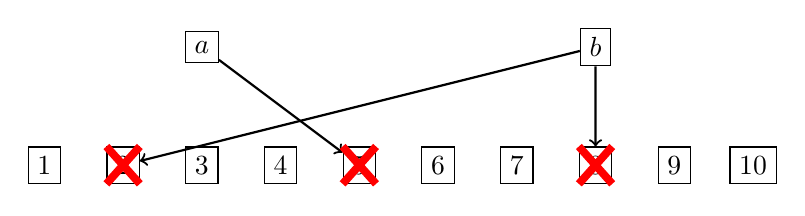
\begin{tikzpicture}
\node[draw] (a) {$a$};
\node[draw] (b) [right of=a,node distance=5cm] {$b$};

\node[draw] (3) [below of=a,node distance=1.5cm] {3};
\node[draw] (4) [right of=3,node distance=1cm] {4};
\node[draw] (5) [right of=4,node distance=1cm] {5};
\node[draw] (6) [right of=5,node distance=1cm] {6};
\node[draw] (7) [right of=6,node distance=1cm] {7};
\node[draw] (8) [right of=7,node distance=1cm] {8};
\node[draw] (9) [right of=8,node distance=1cm] {9};
\node[draw] (10) [right of=9,node distance=1cm] {10};
\node[draw] (2) [left of=3,node distance=1cm] {2};
\node[draw] (1) [left of=2,node distance=1cm] {1};

\draw[->,thick] (a) -- (5);
\draw[->,thick] (b) -- (8);
\draw[->,thick] (b) -- (2);

\draw[red, line width=1mm]
(5.south west) -- (5.north east)
(5.south east) -- (5.north west);

\draw[red, line width=1mm]
(8.south west) -- (8.north east)
(8.south east) -- (8.north west);

\draw[red, line width=1mm]
(2.south west) -- (2.north east)
(2.south east) -- (2.north west);
\end{tikzpicture}
}
\end{center}

Continue this process until all elements of the output alphabet have been
used.

\begin{center}
\resizebox {\columnwidth} {!} {
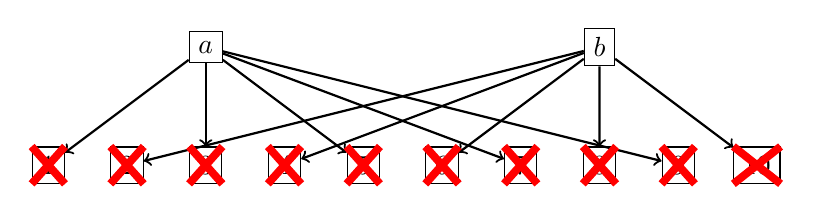
\begin{tikzpicture}
\node[draw] (a) {$a$};
\node[draw] (b) [right of=a,node distance=5cm] {$b$};

\node[draw] (3) [below of=a,node distance=1.5cm] {3};
\node[draw] (4) [right of=3,node distance=1cm] {4};
\node[draw] (5) [right of=4,node distance=1cm] {5};
\node[draw] (6) [right of=5,node distance=1cm] {6};
\node[draw] (7) [right of=6,node distance=1cm] {7};
\node[draw] (8) [right of=7,node distance=1cm] {8};
\node[draw] (9) [right of=8,node distance=1cm] {9};
\node[draw] (10) [right of=9,node distance=1cm] {10};
\node[draw] (2) [left of=3,node distance=1cm] {2};
\node[draw] (1) [left of=2,node distance=1cm] {1};

\draw[->,thick] (a) -- (5);
\draw[->,thick] (b) -- (8);
\draw[->,thick] (b) -- (2);
\draw[->,thick] (a) -- (1);
\draw[->,thick] (a) -- (3);
\draw[->,thick] (a) -- (7);
\draw[->,thick] (a) -- (9);
\draw[->,thick] (b) -- (4);
\draw[->,thick] (b) -- (6);
\draw[->,thick] (b) -- (10);

\draw[red, line width=1mm]
(5.south west) -- (5.north east)
(5.south east) -- (5.north west);

\draw[red, line width=1mm]
(8.south west) -- (8.north east)
(8.south east) -- (8.north west);

\draw[red, line width=1mm]
(2.south west) -- (2.north east)
(2.south east) -- (2.north west);

\draw[red, line width=1mm]
(1.south west) -- (1.north east)
(1.south east) -- (1.north west);

\draw[red, line width=1mm]
(3.south west) -- (3.north east)
(3.south east) -- (3.north west);

\draw[red, line width=1mm]
(4.south west) -- (4.north east)
(4.south east) -- (4.north west);

\draw[red, line width=1mm]
(6.south west) -- (6.north east)
(6.south east) -- (6.north west);

\draw[red, line width=1mm]
(7.south west) -- (7.north east)
(7.south east) -- (7.north west);

\draw[red, line width=1mm]
(9.south west) -- (9.north east)
(9.south east) -- (9.north west);

\draw[red, line width=1mm]
(10.south west) -- (10.north east)
(10.south east) -- (10.north west);
\end{tikzpicture}
}
\end{center}

After all elements from the output alphabet have been used, the encoding table
is composed of all of the choices made:

\begin{center}
\begin{tabular}{|c|c|}
\hline
Symbol & Possible Length Values \\
\hline
$a$ & 1, 3, 5, 7, 9 \\
\hline
$b$ & 2, 4, 6, 8, 10 \\
\hline
\end{tabular}
\end{center}
\end{example}

\begin{example}[Simple Message Encoding Example]
In this example, we will use tweet lengths up to 10, i.e.\ we will use
$\mathbb{N}_{10} = \{1, 2, \ldots, 10\}$ instead of $\tl$.  We will use $\Sigma
= \{a, b\}$ and $\mathcal{X}^* = \{x\}^+$, i.e.\ secret messages will be composed
of combinatiosn of $a$ and $b$ and cover messages will be strings of $x$.

Suppose we want to send the secret message $m = abba$ using the simple
\ttf{Encode} map from example \ref{ex:methodology:twittercc:stego:encoding}.
First, the message
is broken in to the sequence of symbols $a, b, b, a$.  The \ttf{Encode} function
will then map each symbol to a possible length value, e.g.\ 3, 6, 2, 3.  Note
that because each input symbol from $\Sigma$ can map to more than one length
value from $\mathbb{N}_{10}$, the same symbol may or may not be mapped to the
same length value in any given message.  The \ttf{Generate} function will then
create cover messages that match these length values from the set of possible
cover messages $\mathcal{X}^*$: $xxx, xxxxxx, xx, xxx$.  Each cover message
would then be posted to a Twitter account in the order of the original secret
message.  The \ttf{Extract} function on the recipient's side would then take the
tweets in the posted (chronological) order, returning the length values 3, 6, 2,
3.  The \ttf{Decode} function can then apply the same map as the \ttf{Encode}
function and reconstruct the original message $abba$.
\end{example}

This system is generic in that it can be used with many possible input
alphabets, e.g.\ the  English alphabet or
arbitrary half-byte values (0x0, 0x1, \ldots, 0xF).  The English alphabet
allows sending simple messages.  The half-byte alphabet allows sending arbitrary
binary data by splitting each byte of the input data in half and sending each
half as one symbol of the message.  It is impossible to send an entire byte in
one message using this system because the maximum tweet length is only 140
characters.  We chose half-bytes because it is easy to deconstruct and
reconstruct the original bytes and because it is a relatively small alphabet
with only 16 symbols, so it is possible to map each input symbol to almost 10
different tweet length values.  To obtain symbol frequencies for the half-byte
values, it would be best to empirically sample the types of data being sent
across the channel because, in general, each value would likely have an equal
weight.  If the specific type of data being sent is biased toward certain byte
values, that should be considered when weighting the alphabet.

The botnet command and control diagram for this system resembles the diagram
for a centralized botnet, as shown in figure \ref{fig:methodology:twittercc:botnet-diagram}.
A botmaster controls one or more Twitter accounts that have tweets containing
the commands and the bots read from these accounts.

\begin{figure}
\centering
\resizebox {\columnwidth} {!} {
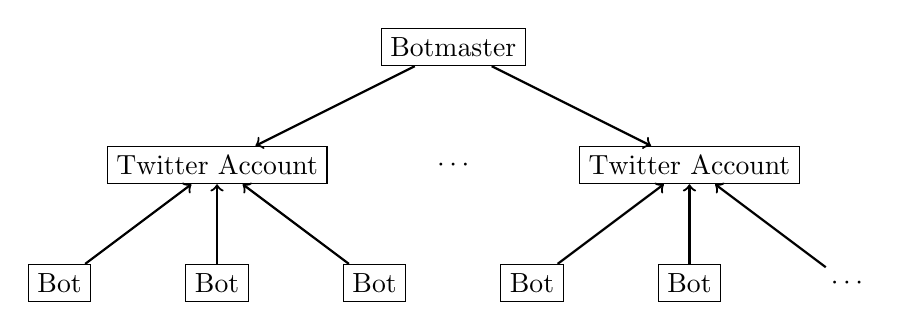
\begin{tikzpicture}
    \node[draw] (m1) {Bot};
    \node[draw] (m2) [right of=m1,node distance=2cm] {Bot};
    \node[draw] (m3) [right of=m2,node distance=2cm] {Bot};
    \node[draw] (m4) [right of=m3,node distance=2cm] {Bot};
    \node[draw] (m5) [right of=m4,node distance=2cm] {Bot};

    \node[draw] (cc1) [above of=m2,node distance=1.5cm] {Twitter Account};
    \node (ccdots) [right of=cc1,node distance=3cm] {$\cdots$};
    \node[draw] (cc2) [above of=m5,node distance=1.5cm] {Twitter Account};
    \node[draw] (m) [above of=ccdots,node distance=1.5cm] {Botmaster};

    \draw[->,thick] (m1) -- (cc1);
    \draw[->,thick] (m2) -- (cc1);
    \draw[->,thick] (m3) -- (cc1);
    \draw[->,thick] (m4) -- (cc2);
    \draw[->,thick] (m5) -- (cc2);
    \node (dots) [right of=m5,node distance=2cm] {$\cdots$};
    \draw[->,thick] (dots) -- (cc2);

    \draw[->,thick] (m) -- (cc1);
    \draw[->,thick] (m) -- (cc2);
\end{tikzpicture}
}
\caption{The botnet C\&C diagram for the system.}
\label{fig:methodology:twittercc:botnet-diagram}
\end{figure}

\subsubsection{The Tweet Generator}
\label{subsec:methodology:twittercc:tweet-gen}

The \ttf{Generate} function is one of the most challenging aspects of this type
of stego system.  As discussed in \cite{steganalysis}, generating appropriate
and plausible cover messages for a stego system is a non-trivial problem.  In this
system, the generator must be capable of generating messages that can convince a
reader of the Twitter account page that they are viewing regular tweets.  This
component has the largest impact on the detectability of the channel.  In
essence, the generator must pass a simplified Turing test.  Twitter bots are not
a new phenomenon, and in fact several bots were created that successfully
convinced other users that they were real people \cite{realboy}.  Additionally,
chat bots exist, such as Cleverbot\footnote{\url{http://www.cleverbot.com/}}
which are reasonably successful \cite{dialogue-system}.  However, aside from
competent English skills, the generator must utilize the ``language of Twitter''
that consists of many
retweets\footnote{\url{https://support.twitter.com/articles/77606-faqs-about-retweets-rt}}
and
hashtags\footnote{\url{https://support.twitter.com/articles/49309-using-hashtags-on-twitter}}.
We consider a strong generator out of the scope of this work, but we leverage the collected Twitter data to create a Twitter language model
based on tweet contents that can be used to generate new tweets.

\subsubsection{Posting to Twitter}
\label{subsec:methodology:twittercc:posting}

Along with the \ttf{Encode}, \ttf{Generate}, \ttf{Extract}, and \ttf{Decode}
functions, we need a system that can post to Twitter.
This is easy to do for testing purposes thanks to Twitter's official
API\footnote{\url{https://dev.twitter.com/docs/api}} and a third party Java
library, Twitter4J\footnote{\url{http://twitter4j.org}}.
For a real botnet scenario, the implementer would likely write their own system
that uses raw HTTP requests because the Twitter API requires authentication of
every call, detects the posting method, and limits the number of posts allowed
for each account.  However, because this would violate Twitter's terms of use, we
will only post tweets using the official API and abide by all limitations
for testing.  Now that the rest of the components have been explained, a more
complete example will be presented.

\begin{example}[Complete Example]
In this example, we will use the full range of tweet lengths $\tl$.  We will use
$\Sigma = \{A, B, \ldots, Z\}$ (the English alphabet), and $\mathcal{X}^*$ as a
pre-constructed list of various proverbs and phrases of lengths ranging from one
to 140.  The \ttf{Generate} function will lookup an appropriate phrase for each
length message provided by the \ttf{Encode} function.  Table
\ref{tab:real-encode} shows a portion of a generated encoding map from English letters to
tweet lengths.  The weights shown in the second column are taken as letter
frequencies\footnote{\url{http://www.math.cornell.edu/~mec/2003-2004/cryptography/subs/frequencies.html}}.
Those weights were used to decide the number of entries for each letter in the
third column.  

Suppose we want to send the message $FOO$.  First, the message is separated in
to the sequence of symbols $F, O, O$.  Each is passed to the \ttf{Encode}
function, which chooses appropriate lengths, e.g.\ 61, 35, 121.  The
\ttf{Generate} function then generates tweets and they are posted to Twitter, as
shown in figure \ref{fig:twitter-posts-foo}.  The figure should be read from
bottom up, because the newer messages are posted on top of the older messages.
The account shown is a test account created for this work.  The recipient then
reads these tweets, obtains the lengths, then uses \ttf{Decode} with the same
table as was used for the \ttf{Encode} process to get the original message.
\end{example}

\begin{table}
\centering
\begin{tabular}{|c|c|p{5.2cm}|}
\hline
Symbol & Weight & Encoding \\
\hline
A & 14810 & 32, 16, 19, 131, 84, 37, 106, 140, 76, 111\\
\hline
B & 2715 & 105, 138, 67 \\
\hline
C & 4943 & 75, 36, 125, 46, 62\\
\hline
F & 4200 & 17, 122, 61, 87\\
\hline
 \ldots & \ldots & \ldots \\
\hline
O & 14003 & 35, 121, 43, 107, 92, 12\\
\hline
 \ldots & \ldots & \ldots \\
\hline
\end{tabular}
\caption{Sample encoding map example for a few English alphabets.}
\label{tab:real-encode}
\end{table}

\begin{figure}
\centering
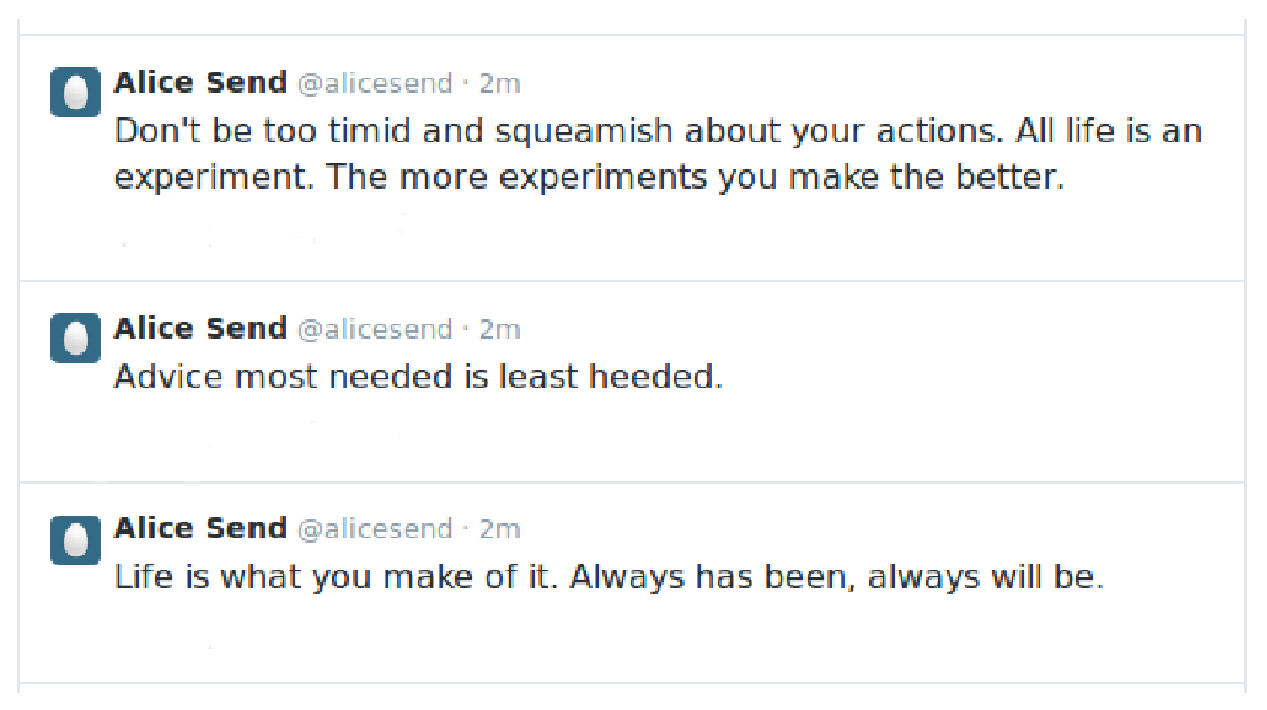
\includegraphics[width=\columnwidth]{foo_test.eps}
\caption{Example showing posted tweets for secret message $FOO$.}
\label{fig:twitter-posts-foo}
\end{figure}

\subsubsection{The Botnet Command and Control Language}
\label{sec:methodology:botnet-cc-lang}

The stego system described in section \ref{subsec:methodology:twittercc:stego} can be
used with an arbitrary input alphabet as long as its size is not larger than the
tweet length range (up to 140 characters), so for botnet command and control we
have developed a language that can be mapped to tweet lengths and interpreted to
execute botnet commands.  We have included some common botnet commands as described
in \cite{twitter-botnet}.  The weights were decided somewhat arbitrarily, because
in a real scenario the botmaster would tailor the weights based on which
commands they believe that they are likely to send most often.  In this case,
We are assuming the byte values (indices 0 to 15) are more likely, because for
some commands arguments must be sent using these.  We don't assume any single
command is more likely than another.

\begin{table}[h]
\centering
\begin{tabular}{|l|l|p{5cm}|}
\hline
Index & Weight & Description \\
\hline
0 & 25 & Literal hex value 0 \\
\hline
1 & 25 & Literal hex value 1 \\
\hline
2 & 25 & Literal hex value 2 \\
\hline
\ldots & \ldots &\ldots \\
\hline
16 & 5 & Take screenshot \\
\hline
17 & 5 & Shutdown computer \\
\hline
18 & 5 & Reboot computer \\
\hline
19 & 5 & Perform DoS attack to IPv4 address in next 4 bytes sent \\
\hline
20 & 5 & Stop DoS attack \\
\hline
21 & 5 & Download and execute file from address in next $k$ bytes (until delimiter) \\
\hline
22 & 1 & Message delimiter \\
\hline
\end{tabular}
\caption{Botnet command and control language for use with the stego system.}
\label{tab:botnet-cc-lang}
\end{table}

\subsubsection{Username Generation using \\Markov Chains}
\label{sec:methodology:usernames}

It is necessary to have a system for generating user names from an initial
seed so that if the original botmaster account is blocked, they can start
a new account and the bots can also generate the new account name and begin
reading from it.  To do this, we employ Markov chains \cite{Markov-chains}.
The Markov chain being used can generate strings of letters, numbers, and
underscores and is trained using an existing corpus of such text (in our case,
a collection of verified Twitter usernames). 

To use this Markov chain for generating a sequence of usernames, both the
bot and botmaster must have the same initial seed.  Using this seed and the
same type of pseudorandom number generator, the
Markov chains will generate the same sequences as long as both bot and
botmaster follow the same procedure.  First, they need to use the random
number generator to choose a user name length.  Second, they use the Markov
chain with this seed to choose
a starting character.  Finally, they generate enough symbols to fit the
length chosen.  If one performs an action out of order, it will affect
the sequences generated after that action.  For example, if the botmaster
chooses the length first while the bot chooses the starting character first,
the sequence generated from the random number generator will cause each to
generate a potentially different length and starting character.

